%%%%%%%%%%%%%%%%%%%%%%%%%%%%%%%%%%%%%%%%%
% Beamer Presentation
% LaTeX Template
% Version 1.0 (10/11/12)
%
% This template has been downloaded from:
% http://www.LaTeXTemplates.com
%
% License:
% CC BY-NC-SA 3.0 (http://creativecommons.org/licenses/by-nc-sa/3.0/)
%
%%%%%%%%%%%%%%%%%%%%%%%%%%%%%%%%%%%%%%%%%

%----------------------------------------------------------------------------------------
%	PACKAGES AND THEMES
%----------------------------------------------------------------------------------------

\documentclass{beamer}
\usepackage{multicol}
\usepackage[russian]{babel}
\mode<presentation> {

% The Beamer class comes with a number of default slide themes
% which change the colors and layouts of slides. Below this is a list
% of all the themes, uncomment each in turn to see what they look like.

%\usetheme{default}
%\usetheme{AnnArbor}
%\usetheme{Antibes}
%\usetheme{Bergen}
%\usetheme{Berkeley}
%\usetheme{Berlin}
%\usetheme{Boadilla}
%\usetheme{CambridgeUS}
%\usetheme{Copenhagen}
%\usetheme{Darmstadt}
%\usetheme{Dresden}
%\usetheme{Frankfurt}
%\usetheme{Goettingen}
%\usetheme{Hannover}
%\usetheme{Ilmenau}
%\usetheme{JuanLesPins}
%\usetheme{Luebeck}
% \usetheme{Madrid}
%\usetheme{Malmoe}
%\usetheme{Marburg}
%\usetheme{Montpellier}
%\usetheme{PaloAlto}
%\usetheme{Pittsburgh}
%\usetheme{Rochester}
%\usetheme{Singapore}
%\usetheme{Szeged}
\usetheme{Warsaw}

% As well as themes, the Beamer class has a number of color themes
% for any slide theme. Uncomment each of these in turn to see how it
% changes the colors of your current slide theme.

%\usecolortheme{albatross}
%\usecolortheme{beaver}
%\usecolortheme{beetle}
%\usecolortheme{crane}
%\usecolortheme{dolphin}
%\usecolortheme{dove}
%\usecolortheme{fly}
%\usecolortheme{lily}
%\usecolortheme{orchid}
%\usecolortheme{rose}
%\usecolortheme{seagull}
%\usecolortheme{seahorse}
%\usecolortheme{whale}
%\usecolortheme{wolverine}

%\setbeamertemplate{footline} % To remove the footer line in all slides uncomment this line
%\setbeamertemplate{footline}[page number] % To replace the footer line in all slides with a simple slide count uncomment this line

%\setbeamertemplate{navigation symbols}{} % To remove the navigation symbols from the bottom of all slides uncomment this line
}

\usepackage{graphicx} % Allows including images
\usepackage{booktabs} % Allows the use of \toprule, \midrule and \bottomrule in tables

%----------------------------------------------------------------------------------------
%	TITLE PAGE
%----------------------------------------------------------------------------------------

\title[Python Intro]{Introduction to Python} % The short title appears at the bottom of every slide, the full title is only on the title page

\author{Sugarkhuu Radnaa} % Your name
\institute[] % Your institution as it will appear on the bottom of every slide, may be shorthand to save space
{
Py4Econ in Ulaanbaatar \\ % Your institution for the title page
\medskip
\textit{py4econ@gmail.com} % Your email address
}
\date{\today} % Date, can be changed to a custom date

\begin{document}

\begin{frame}
\titlepage % Print the title page as the first slide
\end{frame}

\begin{frame}
\frametitle{About the course} % Table of contents slide, comment this block out to remove it
\begin{enumerate}
    \item Basic programming know-hows
    \item Elementary to Intermediate Python
        \begin{itemize}
            \item Python topics covered: data structures, control flow, functions, modules, classes, files, regex, automation, data visualization, web scraping
            \item Python topics not covered: data analysis, web development, ML & AI
        \end{itemize}
    \item Final projects:
        \begin{itemize}
            \item Excel manipulation 
            \item Data cleaning and visualization 
            \item Web scraping & sending automated email
        \end{itemize}
\end{enumerate}
% \tableofcontents % Throughout your presentation, if you choose to use \section{} and \subsection{} commands, these will automatically be printed on this slide as an overview of your presentation
\end{frame}

%----------------------------------------------------------------------------------------
%	PRESENTATION SLIDES
%----------------------------------------------------------------------------------------

\begin{frame}
    \frametitle{Week 1: Learning objectives}
    \begin{enumerate}
        \item Overview of Python 
        \item Computer basics
        \item Communities
        \item Folder structures, Path, Shell
        \item Python / Anaconda
        \item Text editor, notebook, IDE
        \item Git & Github
        \item Coding best practices
    \end{enumerate}
\end{frame}

%------------------------------------------------
\section{Background} 
%------------------------------------------------

% \subsection{Subsection Example} % A subsection can be created just before a set of slides with a common theme to further break down your presentation into chunks

\begin{frame}
\frametitle{Ask ask and ask!}
\centering
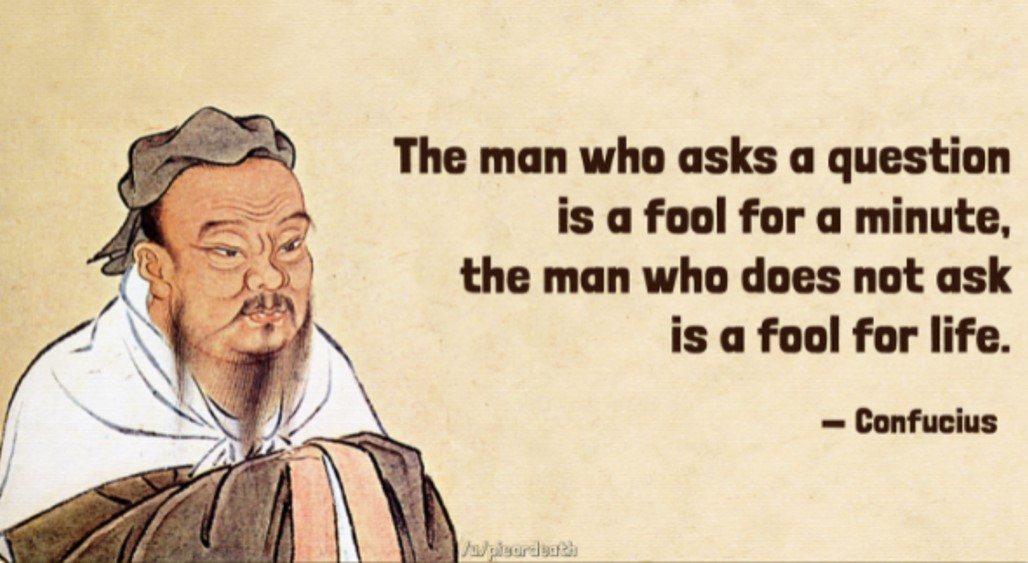
\includegraphics[scale = 0.5]{figures/confucius.jpg}
\end{frame}

\begin{frame}
    \frametitle{Why Python?}
    \centering
    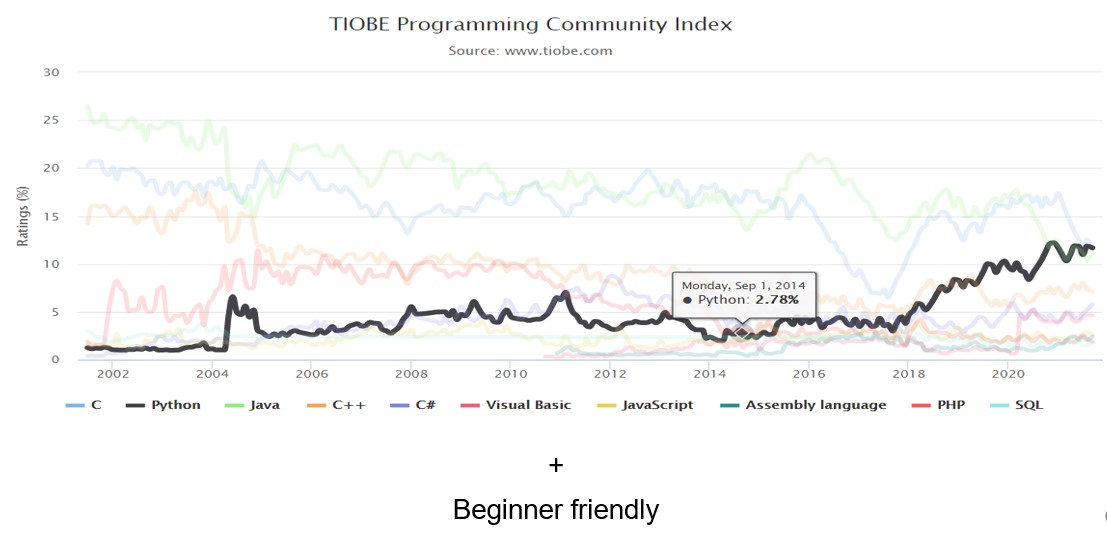
\includegraphics[scale = 0.5]{figures/trend_python.jpg}
\end{frame}

\begin{frame}
    \frametitle{Popular applications of Python}
    \begin{enumerate}
        \item Data science and data visualization
        \item Machine learning & AI
        \item Scientific computing (incl. Financial modelling)
        \item Web & Game development
        \item Desktop applications & Software & GUI
        \item Automation
    \end{enumerate}
\end{frame}

\begin{frame}
    \frametitle{Python was first released in 1991}
    \centering
    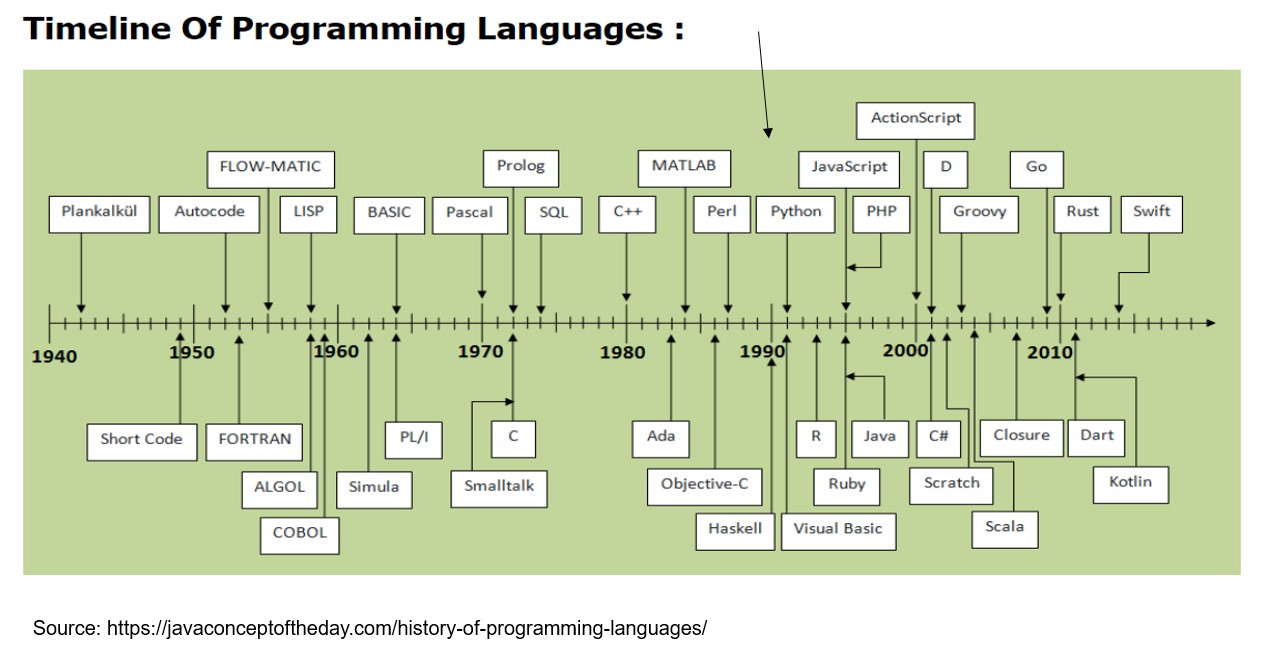
\includegraphics[scale = 0.4]{figures/timeline_lang.jpg}
\end{frame}

\begin{frame}
    \frametitle{Computer basics}
    \centering
    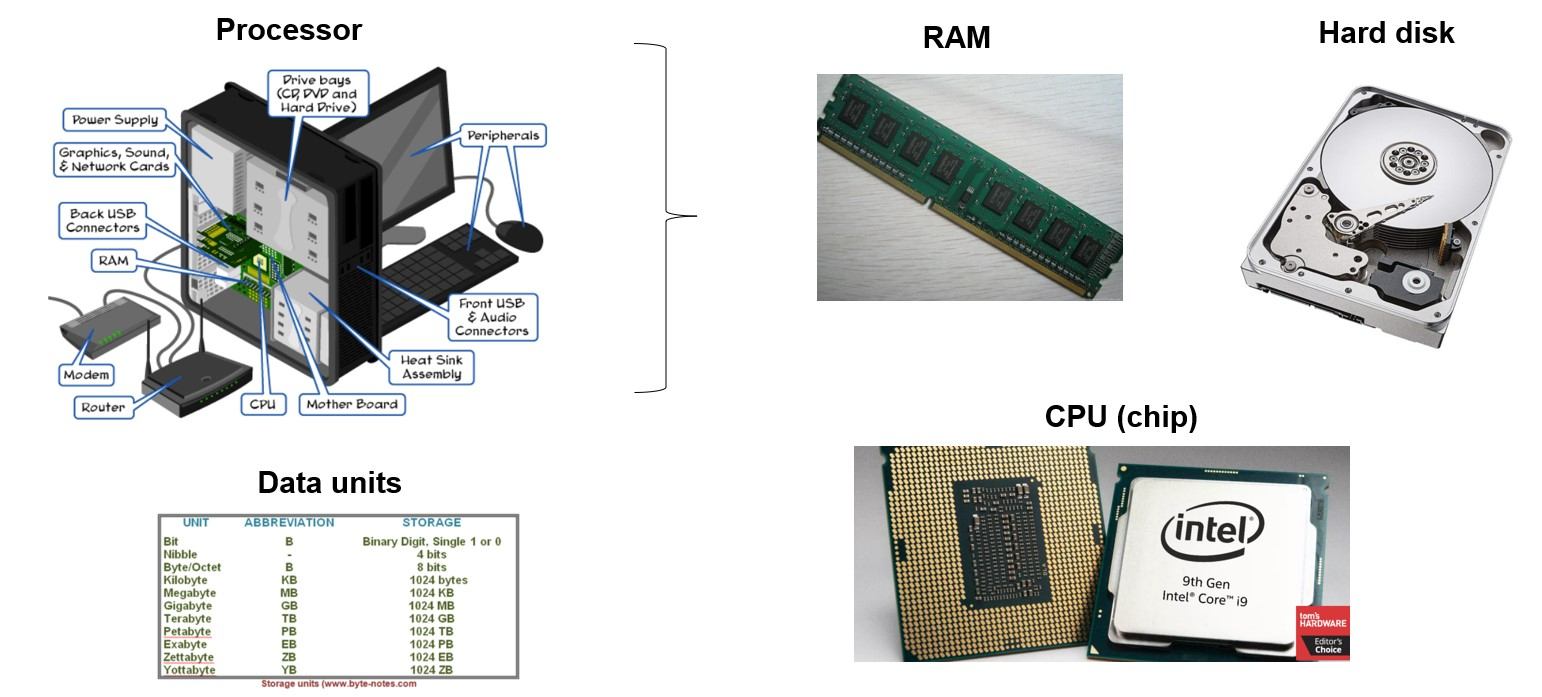
\includegraphics[scale = 0.35]{figures/computer.jpg}
\end{frame}

\begin{frame}
    \frametitle{Operating systems}
    \centering
    
\includegraphics[scale = 0.5]{figures/os.jpg}
\end{frame}

\begin{frame}
    \frametitle{Communities and learning platforms}
    \begin{multicols}{2}
        \begin{enumerate}
            \item Python - Official
            \item Stack overflow - Forum
            \item Medium - Blog
            \item Towardsdatascience - Blog
            \item Tutorialspoint
            \item Geek for geeks
            \item W3schools
            \item Real Python
            \item Programiz
            \item Kaggle - Competition and Learning resource
            \item DrivenData
            \item TopCoder
            \item DataHack
        \end{enumerate}
    \end{multicols}
\end{frame}

%------------------------------------------------
\section{Programming basics} 
\frame{\tableofcontents[currentsection]}
%------------------------------------------------

\begin{frame}
    \frametitle{What is a programming language?}
    A programming language is a formal language comprising a set of strings 
    that produce various kinds of machine code output.
    Wikipedia \\
    \centering
    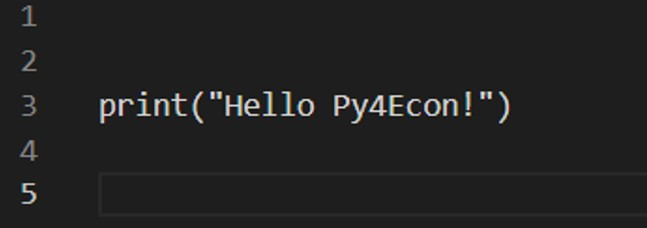
\includegraphics[scale = 0.3]{figures/hello.jpg}   
\end{frame}

\begin{frame}
    \frametitle{Must-have basics for a good programmer}
    \begin{itemize}
        \item Data Structure and Algorithm
        \item A Version Control Tool (Git)
        \item One Text Editors (VScode)
        \item IDEs (Spyder or Pycharm)
        \item Database and SQL
        \item UNIX (Linux)
        \item An OOP Programming language (C++, Java or Python)
        \item One Scripting language (automation)
        \item Networking basics
        \item \textit{Cloud Platform (AWS, GCP, or Azure)}
        \item \textit{Containers (Docker and Kubernetes)}
    \end{itemize}
\end{frame}

\begin{frame}
    \frametitle{Folder structure}
    \centering
    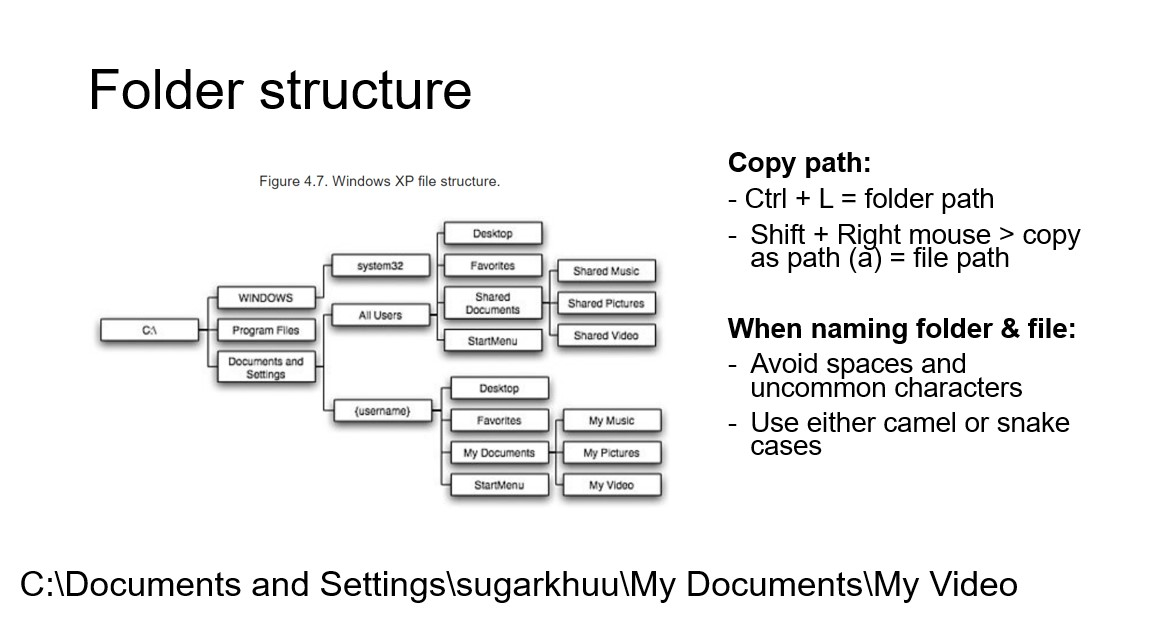
\includegraphics[scale = 0.5]{figures/folder.jpg}
\end{frame}

\begin{frame}
    \frametitle{Command line interpreters/Shells}
    \centering
    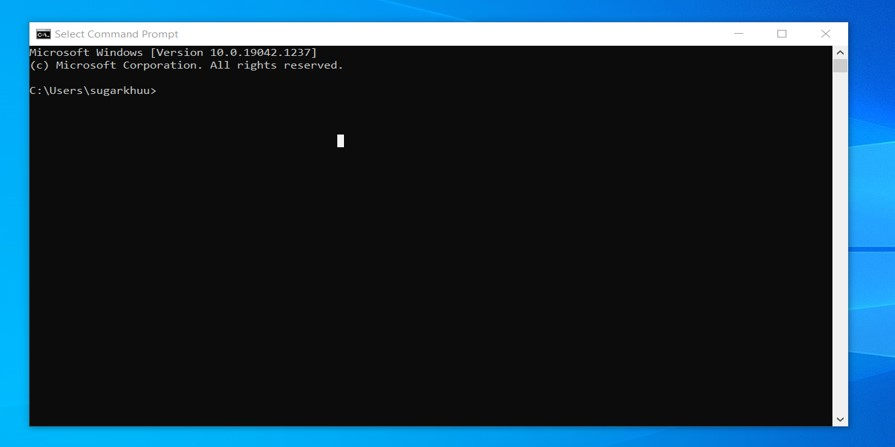
\includegraphics[scale = 0.5]{figures/bash.jpg}

    You are able to control your computer through commanding
    the OS from terminals. More powerful and flexible than usual GUI way of doing things \\

    \begin{itemize}
        \item Windows: Command prompt, Powershell. More recently, Windows Terminal \\
        \item Linux: Bash
        \item Mac: Terminal (zsh)
    \end{itemize}
\end{frame}

\begin{frame}
    \frametitle{Common CMD/Bash commands}
    \begin{itemize}
        \item cd [cd] – change directory. /? - help
        \item dir [ls] – directory content
        \item copy [cp] – copy file
        \item ren [mv] – rename file
        \item del [rm] – delete file
        \item mkdir [mkdir] – create new folder
        \item exit [exit] - close terminal
        \item cls [ctrl+L] – clear terminal
    \end{itemize}
\end{frame}

\begin{frame}
    \frametitle{Path (environment variable)}
    \centering
    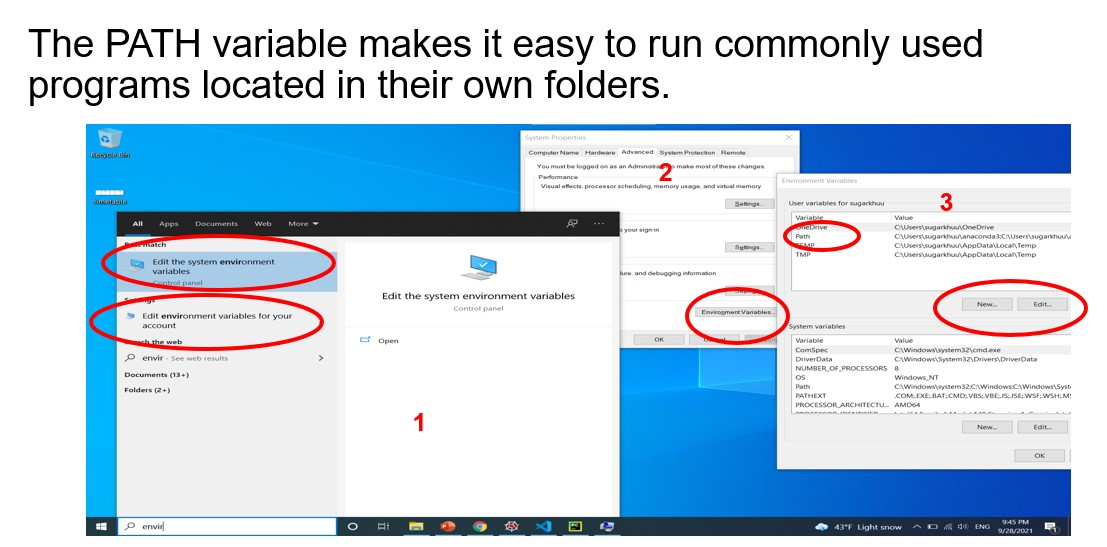
\includegraphics[scale = 0.5]{figures/path.jpg}
\end{frame}

\begin{frame}
    \frametitle{Getting Python}
    \centering
    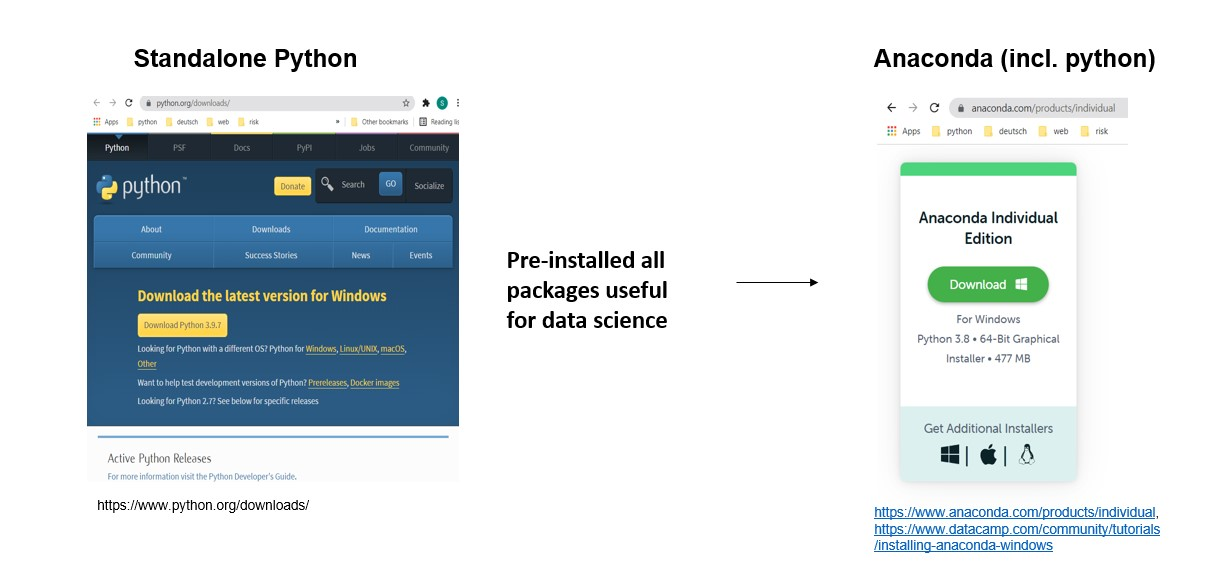
\includegraphics[scale = 0.5]{figures/getpython.jpg}
\end{frame}

\begin{frame}
    \frametitle{Possible to use Python in many environments}

    \begin{enumerate}
        \item Terminal
        \item IDEs – Spyder or Pycharm (IntelliJ), VScode
        \item Notebook -  (\href{https://github.com/susanli2016/Machine-Learning-with-Python}
        {Jupyter notebook})
    \end{enumerate}
\end{frame}

\begin{frame}
    \frametitle{Python basic concepts for today:}

    \begin{itemize}
        \item Basic syntax
        \item Basic operators
        \item Packages (+ pip)
        \item Docstring
        \item Read data
    \end{itemize}
\end{frame}

\begin{frame}
    \frametitle{Using VS code (code editor) for Python}
    \centering
    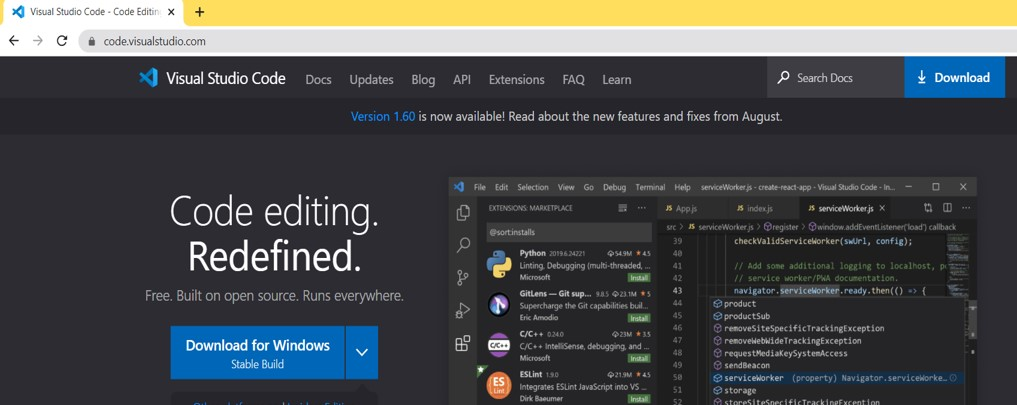
\includegraphics[scale = 0.5]{figures/vscode.jpg}
\end{frame}

\begin{frame}
    \frametitle{Git – Version control system (VCS)}
    \centering
    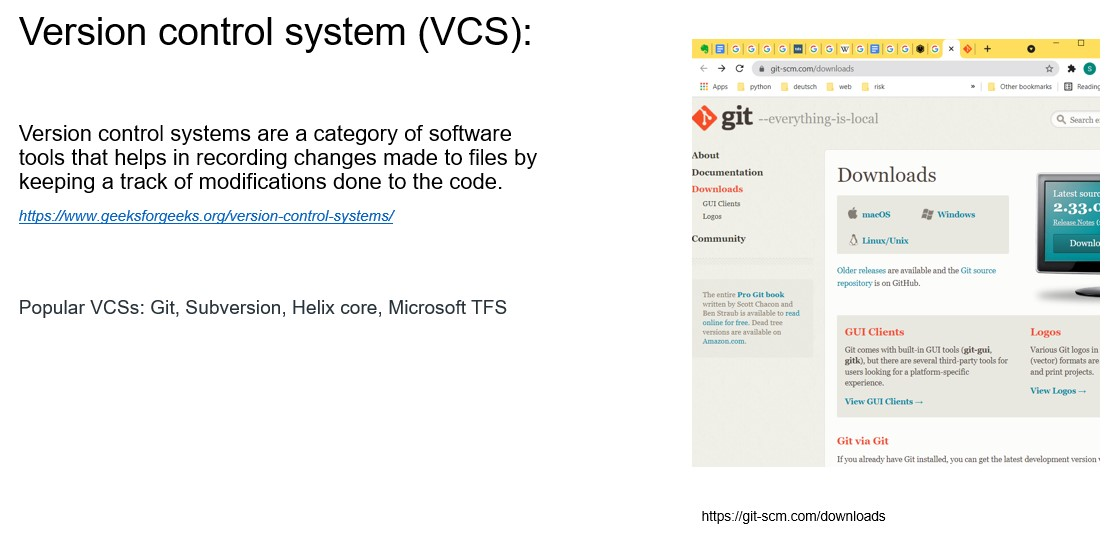
\includegraphics[scale = 0.5]{figures/git.jpg}
\end{frame}

\begin{frame}
    \frametitle{Git – Version control system (VCS)}
    \centering
    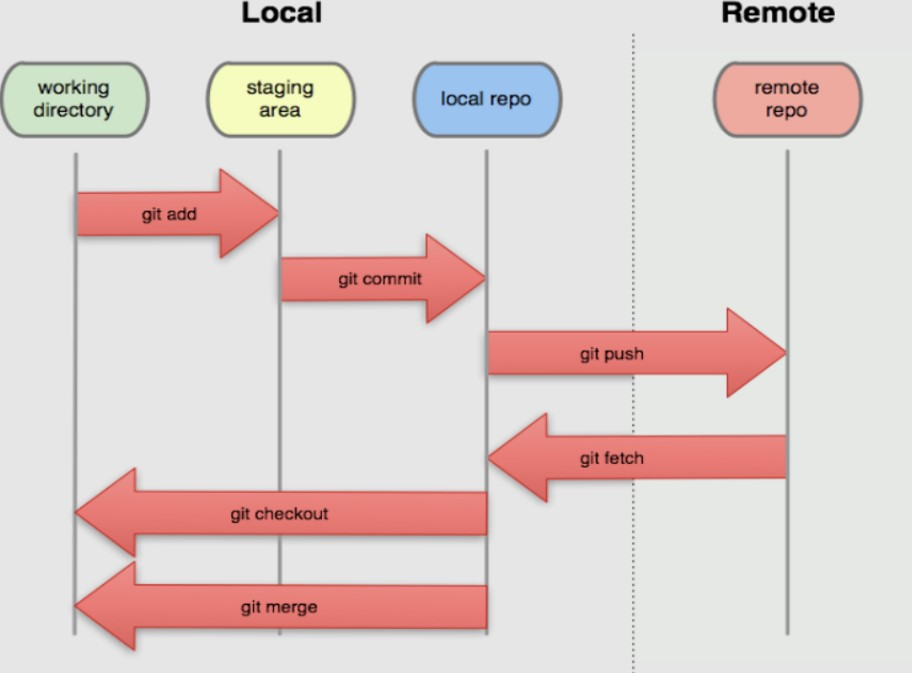
\includegraphics[scale = 0.5]{figures/git_flow.jpg}
\end{frame}

\begin{frame}
    \frametitle{Github – Share everything you want}
    \centering
    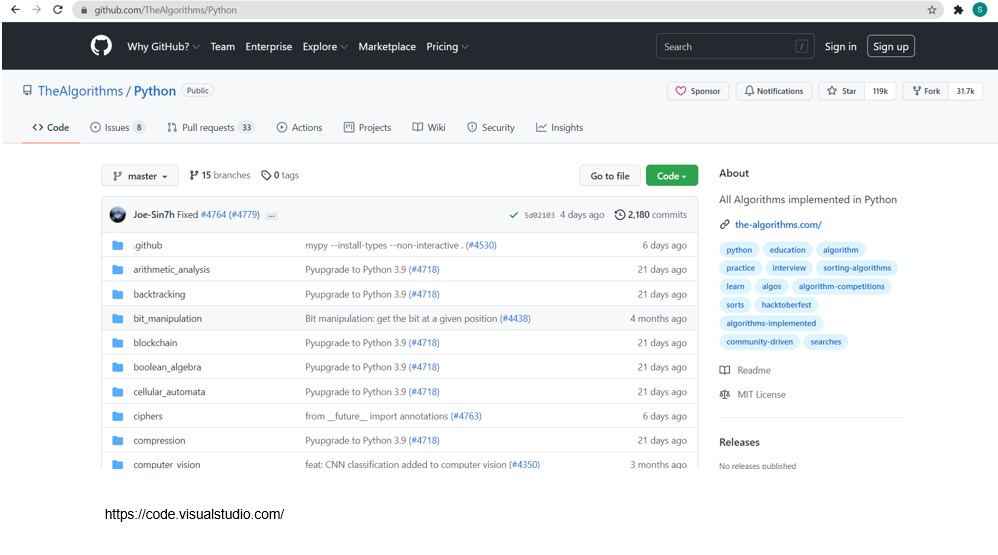
\includegraphics[scale = 0.5]{figures/github.jpg}
\end{frame}

\begin{frame}
    \frametitle{Git bash}
    A unix based commands on Windows (Emulator)
    \centering
    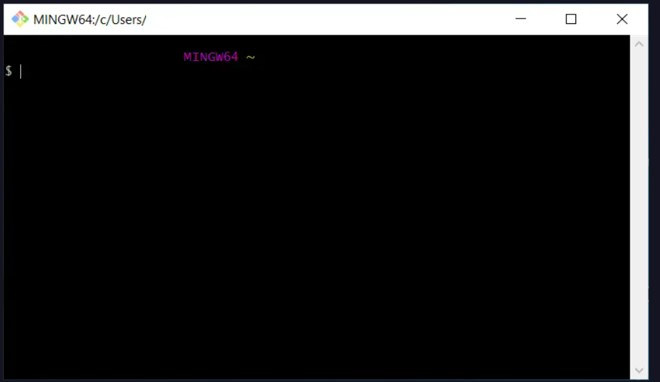
\includegraphics[scale = 0.5]{figures/git_bash.jpg}
\end{frame}

\begin{frame}
    \frametitle{Coding best practices}
    \begin{itemize}
        \item Description of the code
        \item Comments
        \item Simple and short variable name (convention)
        \item Indentation
        \item Commit little by little
        \item Logically consistent and well tested … 
    \end{itemize}
\end{frame}

\begin{frame}
    \frametitle{Homework}
    \begin{enumerate}
        \item Task 1
        \item Task 2
    \end{enumerate}
    Deadline: 18 December, 2021
\end{frame}

\begin{frame}
    \frametitle{Task 1}
    \begin{enumerate}
        \item Create a new repository in your Github
        \item Clone the previous repository to your local machine
        \item Create a Jupyter notebook in the local repo (in your folder)
        \item In the notebook, write a code which asks 5 separate questions and 
        receives the answers from the user (we had an example with only one question
        in the lecture)
        \item Commit and push your changes question by question one at a time
        \item Make sure your code follows the good practice
    \end{enumerate}
\end{frame}

\begin{frame}
    \frametitle{Task 2}
    \begin{enumerate}
        \item Нэг компьютерт хоёр үйлдлийн систем суулгаж болох уу?
        \item Path-д программаа оруулаагүй бол яах вэ?
        \item Фолдерийн нэр нь дундаа зайтай байвал фолдерийг танихад ямар асуудал үүсэх вэ?
        \item Git, Github хоёрын ялгаа юу вэ?
        \item Jupyter notebook IDE мөн үү?
        \item Commit, push хоёрын ялгаа юу вэ?
        \item Push хийхээс өмнө олон дахин commit хийж болох уу?
        \item Commit хийхэд github repo-д access хэрэгтэй юу?
    \end{enumerate}
\end{frame}

\begin{frame}
\Huge{\centerline{Thank you!}}
\end{frame}

%----------------------------------------------------------------------------------------

\end{document} 